\documentclass{beamer} %

%%%BASICS
\usepackage[utf8]{inputenc}
\usepackage{csquotes}
\usepackage{graphicx}
\usepackage{graphics}

\usepackage{caption}
\captionsetup{font=footnotesize}

%%%START THEME SETTINGS


\usetheme{Dresden}

%\usecolortheme{beaver}
\definecolor{beamer@blendedblue}{RGB}{208,132,73}

\setbeamercolor{structure}{fg=beamer@blendedblue}

%\usecolortheme{beamer@blendedblue}

\usefonttheme{professionalfonts}
\setbeamertemplate{itemize item}{\color{beamer@blendedblue}$\blacksquare$}
%%%END THEME SETTINGS

%%%START APA
\usepackage[british]{babel}
\usepackage[backend=biber,style=apa]{biblatex}
\DeclareLanguageMapping{british}{british-apa}
\addbibresource{references.bib}
%% APA citing
%% \cite{t} - Uthor und Richter, 2010
%% \textcite{t} - Uthor und Riter (2010)
%% \parencite{t} - (Uthor & Riter, 2010)
%% \parencite[Chapt.~4]{t} - (Uthor & Riter, 2010, S. 15)
%%%END APA

%---------------------------------------------------



\title[Radiocarbon Dating with MCMC]{Analyzing Radiocarbon Data with Temporal Order Constraints}
\institute[]{Department of Mathematics}
\author[]{Reilly Villanueva}

\date{May 6th, 2016}


\begin{document}
\begin{frame}
	\titlepage

\end{frame}

%------------------------------------------------------
%
%
%\begin{frame}
%
%\begin{centering}
%	Contents
%    \begin{itemize}
%		\item Radiocarbon
%        \item Numerical Integration
%        \item Markov Chain Monte Carlo
%        \item R Tephra Data
%        \item Analysis / Results
%    \end{itemize}
%    
%    \end{centering}
%
%\end{frame}

%--------------------------------------------------------

\begin{frame}
	\frametitle{Calibration Curve}
	\begin{figure}
	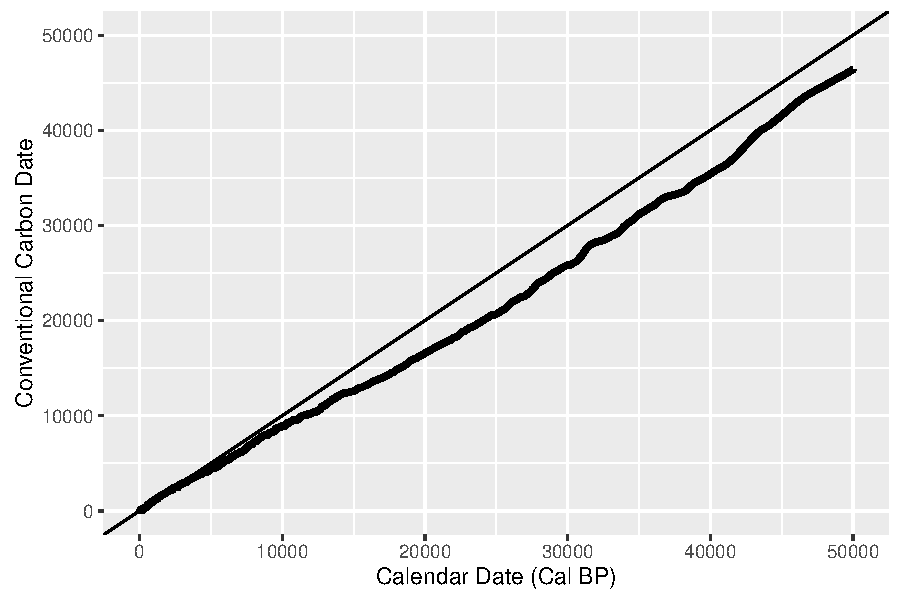
\includegraphics[width=\textwidth]{fullcal}
	\end{figure}

\end{frame}

%----------------------------------------------------------

\begin{frame}
	\frametitle{Calibration Curve}
	\begin{figure}
	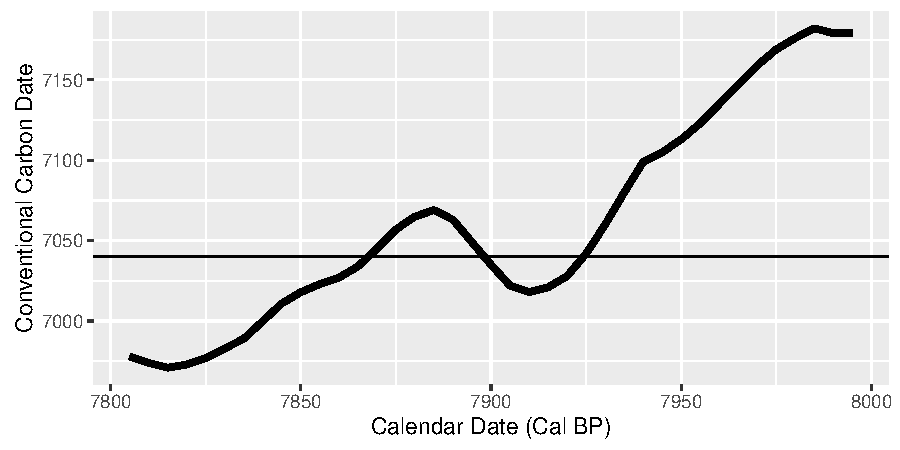
\includegraphics[width=\textwidth]{partcal}
	\end{figure}

\end{frame}

%---------------------------------------------------------

\begin{frame}
	
	\frametitle{Bayes Theorem}
	
	$B$ is an event.
	\hfill \break
	
	$A_1, \dotso, A_n$ is a set of disjoint outcomes.
	
	\[
	P(A_i|B) = \frac{P(B|A_i) P(A_i)}{\sum_{i=1}^n P(B|A_i)P(A_i)} 
	\]	

\end{frame}

%--------------------------------------------------------

\begin{frame}

	\frametitle{Bayes for Probability Densities}
	
	$X$ for conventional carbon dates.
	\hfill \break

	
	$\theta$ for ages of samples.
	
	\[  
	\pi(\theta|x) = \frac{f(x|\theta)\pi(\theta)}{\int f(x|\theta)\pi(\theta) d\theta }
	 \]


\end{frame}

%--------------------------------------------------------

\begin{frame}
	\frametitle{Temporal Order Constraints}
	
	For samples $\alpha_1, \alpha_2, \alpha_3$ as shown

	\begin{center}
	\includegraphics[width=2.5in, height = 2in]{OneSedimentLayer}
	\end{center}
	
	We assume ordered ages: $0 < \theta_1 < \theta_2 <  \theta_3 < 50000$
	
\end{frame}


%---------------------------------------------------------

\begin{frame}

	\frametitle{Numerical Integration}
	Bayes:
	\[  
\pi(\theta|x) = \frac{f(x|\theta)\pi(\theta)}{\int f(x|\theta)\pi(\theta) d\theta }
 \]
	
	Approximating the Integral:
	\[
\int_a^b f(x|\theta)\pi(\theta) d\theta \approx \sum_{i=a}^{b} f(x | \theta_i ) \pi( \theta_i ) \Delta \theta_i
\]

\end{frame}

%--------------------------------------------------------

\begin{frame}
	\frametitle{Markov Chains}
	
	Let $\Theta_i$ be a random variable, and let $\theta_i$ be a single draw from the random variable $\Theta_i$. 
	
	A \textbf{\textit{Markov chain}} is a sequence $\Theta_1, \Theta_2, \dotso$ of random variables where the conditional distribution of $\Theta_{n+1}$ given $\theta_1, \dotso , \theta_n$ depends only on $\theta_n$.
	\hfill \break
	 A sequence of random variables $\Theta_1, \Theta_2, \dotso$ is \textbf{\textit{stationary}} if for every positive integer $k$, the distribution of the $k$-tuple $(\theta_{n+1}, \dotso , \theta_{n+k})$ does not depend on $n$. 
 
	

\end{frame}

%-------------------------------------------------------

\begin{frame}

	\frametitle{Gibbs Sampler}
	

Begin with the Markov chain at state $t$, written as $x^t = (x_1^t,\dotso,x_p^t)$. 

\begin{enumerate}

\item Generate $X_1^{t+1} \sim f_1(x_1 | x_2^t,\dotso,x_p^t)$.
\item Generate $X_2^{t+1} \sim f_2(x_2 | x_1^{t+1},x_3^t,\dotso,x_p^t)$.

$\vdots$

\item [p.] Generate $X_p^{t+1} \sim f_p(x_p|x_1^{t+1},\dotso,x_{p-1}^{t+1})$.

\end{enumerate}

\end{frame}

%--------------------------------------------------------

\begin{frame}

\frametitle{Metropolis-Hastings}

Let $h$ be the (not necessarily normalized) probability density of the stationary distribution we are constructing. 
\begin{enumerate}
\item While at position $x_i$, propose a move to position $y$ having probability density conditioned on $x_i$, written as $q(y | x_i)$.
\item Let $h(x)$ be the density at the sample when $h$ is parameterized by $x$. Compute the Hastings ratio:

\[
r(x_i,y) = \frac{h(y) q(y | x_i)} {h(x_i) q(x_i | y)}.
\]

\item Accept the proposed move with probability $a(x_i, y) = \min(1, r(x_i, y)$. 
\end{enumerate}

\end{frame}


%--------------------------------------------------------

\begin{frame}
	\frametitle{Highest Posterior Density Region}
	\begin{figure}
	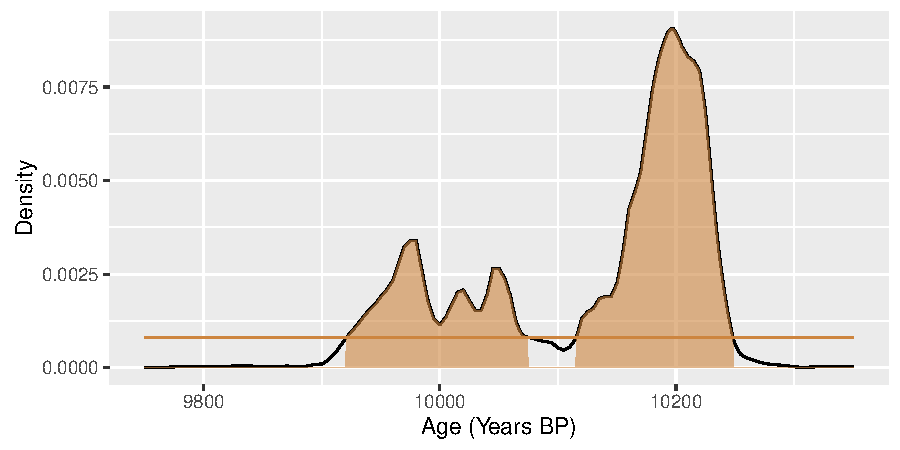
\includegraphics[width=\textwidth]{credintexam}
	\end{figure}

\end{frame}

%----------------------------------------------------------

\begin{frame}
	\frametitle{Proposal Density for Samples with Carbon Dates}
	$\theta_j^i$ is the $i$-th estimate for the $j$-th sample's age and $x_j$ is the radiocarbon date of the $j$-th sample
	
	\[
f(x_{j} | \theta^{i-1}_{j-1}, \theta^{i-1}_{j+1} ) =     
 \begin{cases}
      N(\theta^{i-1}_{j},\sigma^2), & \text{if }\ \frac{\theta^{i-1}_j  - \theta^{i-1}_{j-1}}{2}< \theta^i_j < \frac{\theta^{i-1}_{j+1} - \theta^{i-1}_j}{2}  \\
      0, & \text{otherwise}\ 
    \end{cases}
\]  
	
\end{frame}

%----------------------------------------------------------

\begin{frame}
	\frametitle{Proposal Density for Samples without Carbon Dates}
	
	$z_k$ is the sample without a carbon date
	
	\[
f(z_k | \theta_{k-1}^i, \theta_{k+1}^i) = 
\begin{cases}
	c, & \text{ if }\theta^i_{k-1} < \theta_k^i < \theta^i_{k+1}  \\
	0, & \text{ otherwise}
\end{cases}
\]

where c is some constant.

\end{frame}

%----------------------------------------------------------

\begin{frame}

	\frametitle{R Tephra Data}
	
	\begin{minipage}[l]{.60\textwidth}

	\begin{table}[h]
	%\caption{The data in the R tephra dataset (\cite{samol:2016}).}
\label{tab: data}
\begin{center}
\resizebox{\columnwidth}{!}{%
\begin{tabular}{| c | c | c |}
\hline
 Description& Carbon-14 age & Location relative  \\ 
  & (years BP) & to R tephra \\ \hline \hline
Coniferous needle& 8905$\pm$20& 20.5cm above \\ \hline
Twig& 8920$\pm$60& directly above \\ \hline
Charcoal& 8890$\pm$40& directly under\\ \hline
Peat& 8760$\pm$80& 50cm below \\ \hline
Small twig& 8990$\pm$60& 100cm+ below\\ \hline
	\end{tabular}   }
	\end{center}
	\end{table}
	
	
	\end{minipage}%
	\begin{minipage}{.40\textwidth}
	
	\begin{figure}
	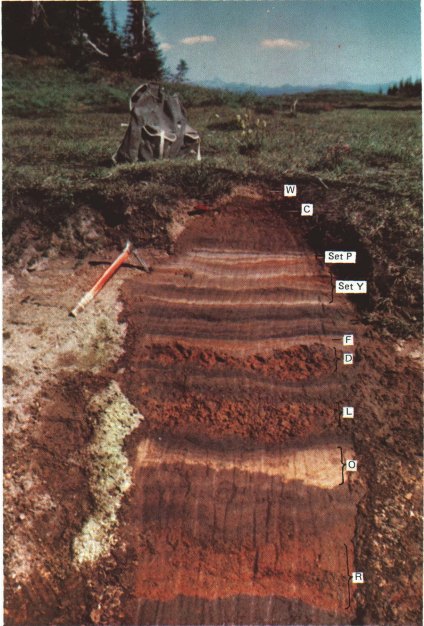
\includegraphics[width = \textwidth]{rainiertephra}
	
	\tiny{Credit: U.S. Geological Survey 
Department of the Interior/USGS}
	\end{figure}
	\end{minipage}
\end{frame}


%-----------------------------------------------------------


\begin{frame}
	\frametitle{Comparing Numerical Integration and MCMC}
	
	\begin{figure}
	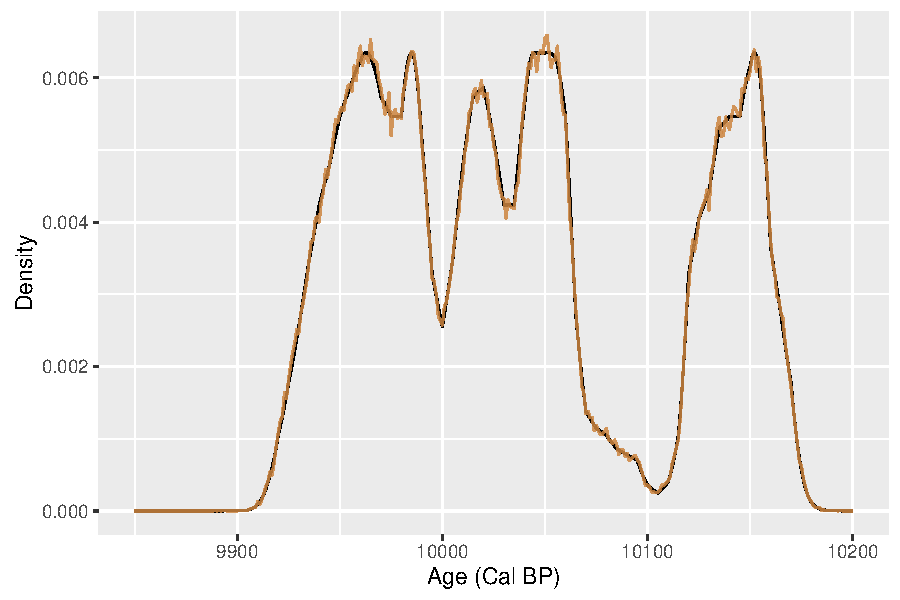
\includegraphics[width=\textwidth]{num&mcmc}
	\end{figure}
\end{frame}

%-----------------------------------------------------------

\begin{frame}
	\frametitle{Posterior Densities}
	\begin{figure}
	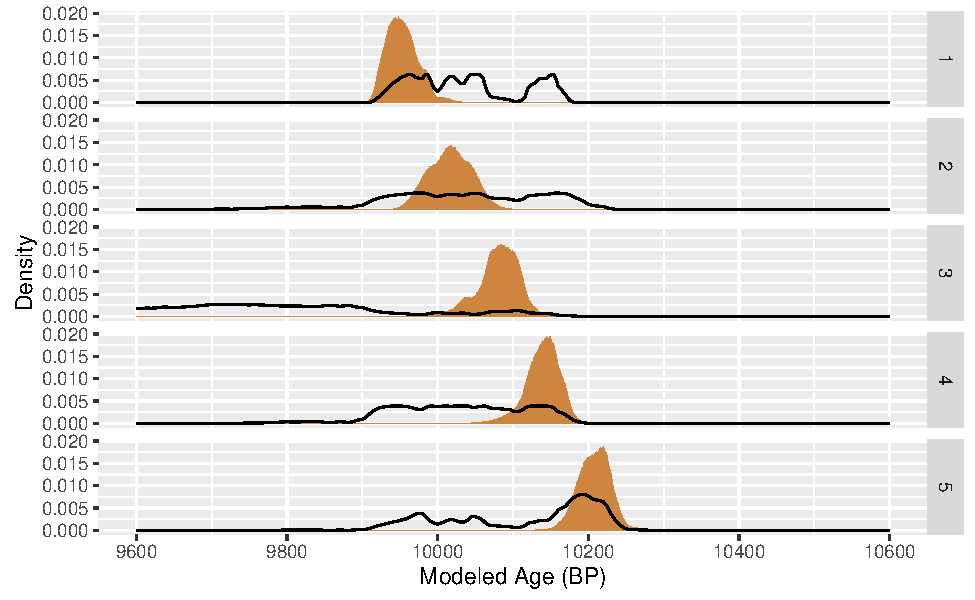
\includegraphics[width=\textwidth]{Fig4Arep}
	\end{figure}
	
\end{frame}


%---------------------------------------------------------

\begin{frame}
	
	\begin{figure}
	\includegraphics[width=\textwidth]{tephstack}
	\end{figure}
	

\end{frame}




\printbibliography

\end{document}